\section*{Results}
\subsection{Free floating depths with varmin optimization (spin-independent)}

\begin{figure}[htbp]
    \centering
    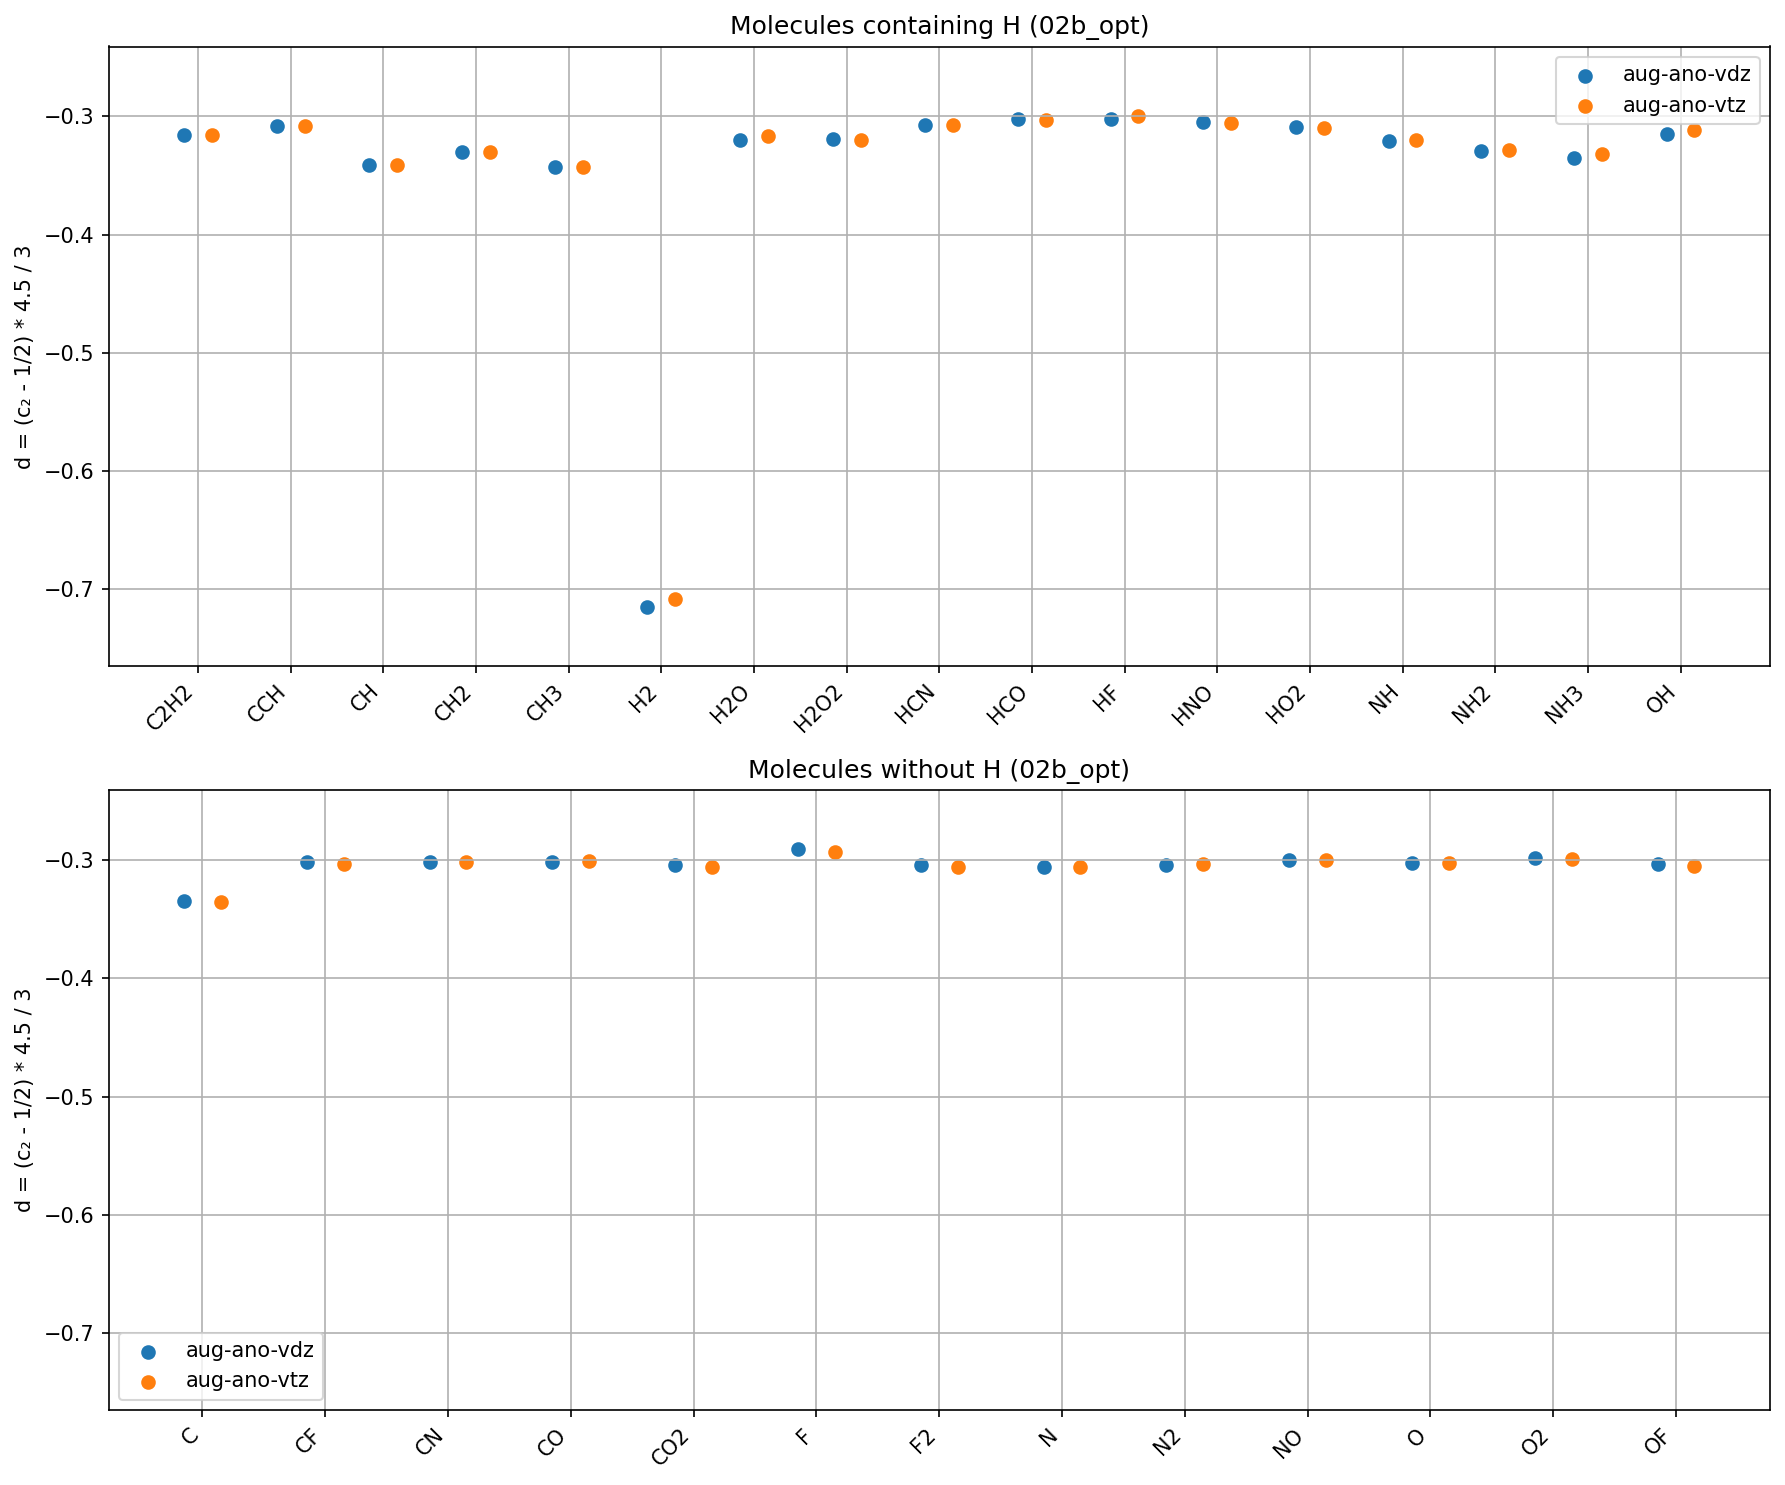
\includegraphics[width=0.6\linewidth]{figures/Free_floating_depths_AE.png}
    \caption{Free floating depths for AE calculations}
    \label{fig:free_varmin_AE}
\end{figure}

\begin{figure}[htbp]
    \centering
    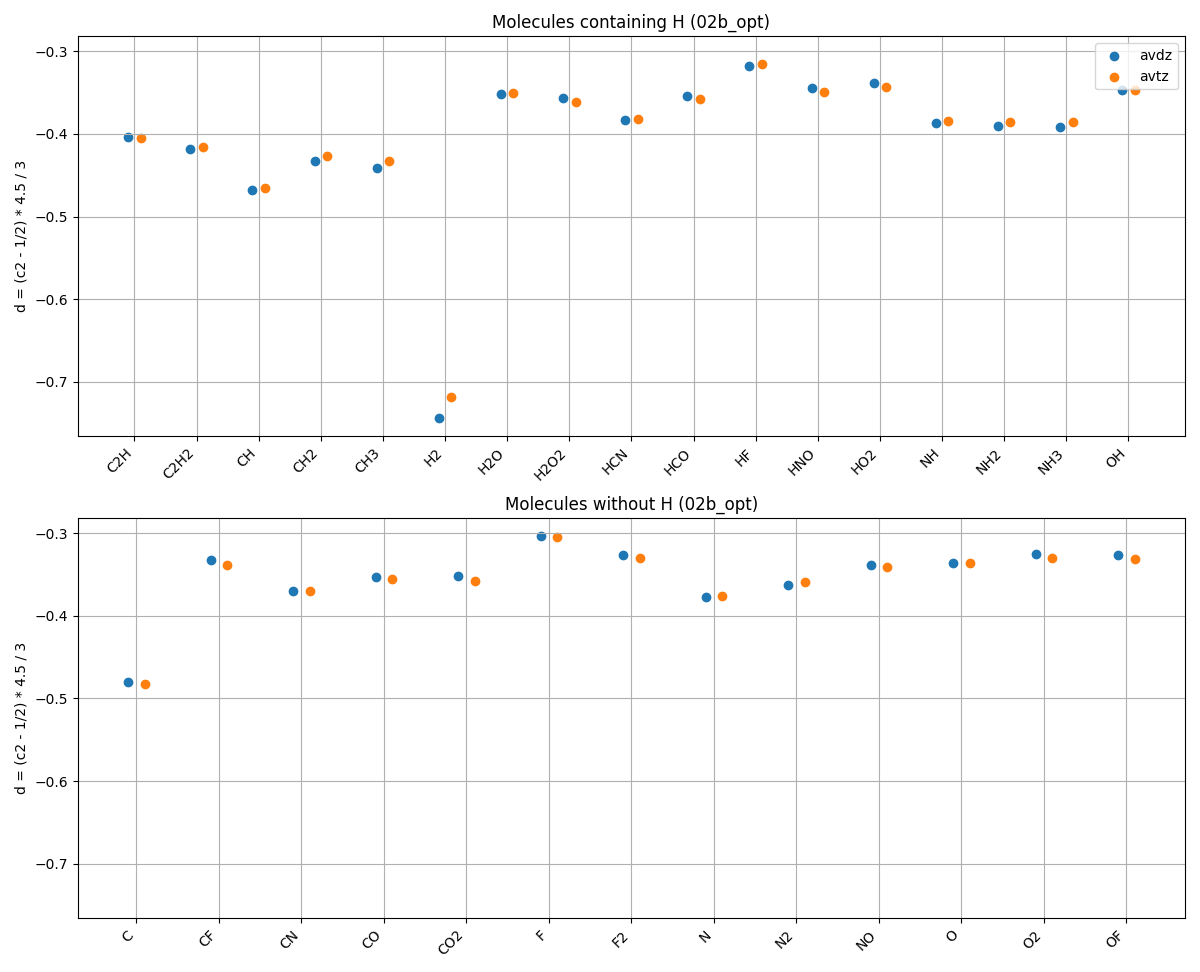
\includegraphics[width=0.6\linewidth]{figures/Free_floating_depths_ECP.png}
    \caption{Free floating depths for ECP calculations}
    \label{fig:free_varmin_ECP}
\end{figure}

\subsection{CCSD(T) energies against heat}

\subsubsection{eCEPP}

\begin{figure}[htbp]
    \centering
    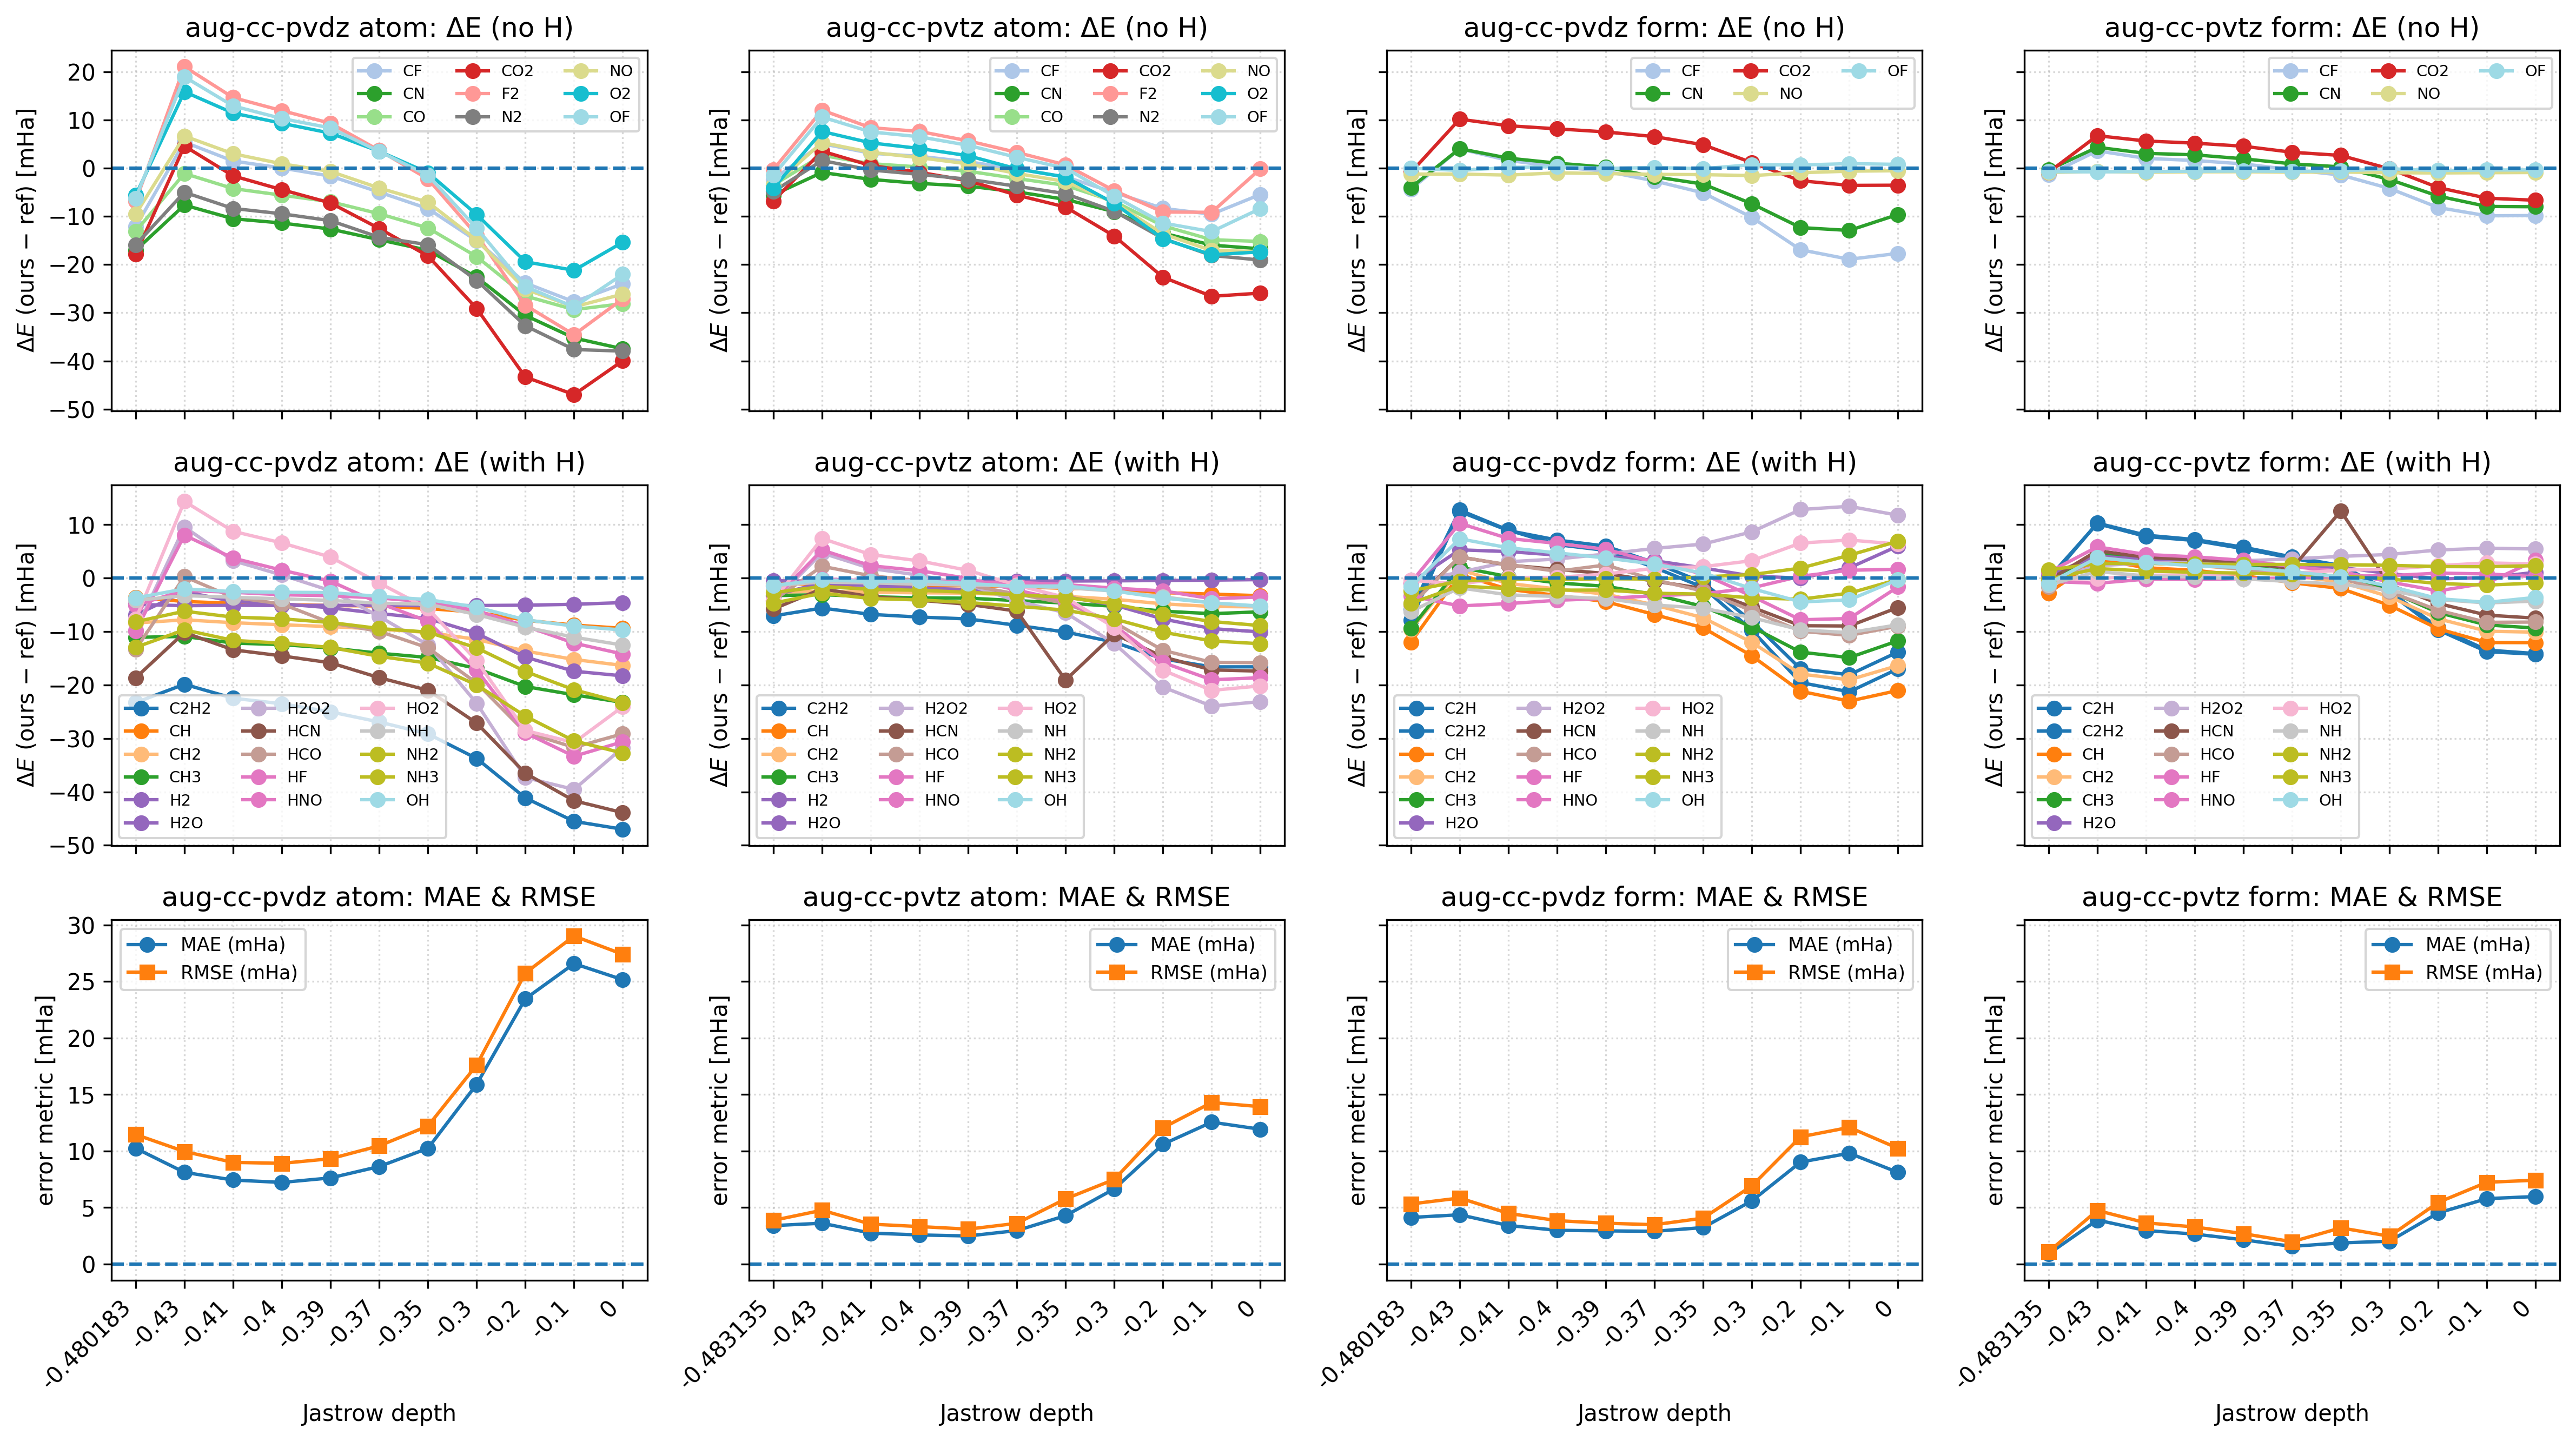
\includegraphics[width=1.1\linewidth]{figures/depth_sweep_eCEPP.png}
    \caption{eCEPP}
    \label{fig:feCEPP depth sweep}
\end{figure}

\subsubsection{ccECP}

\begin{figure}[htbp]
    \centering
    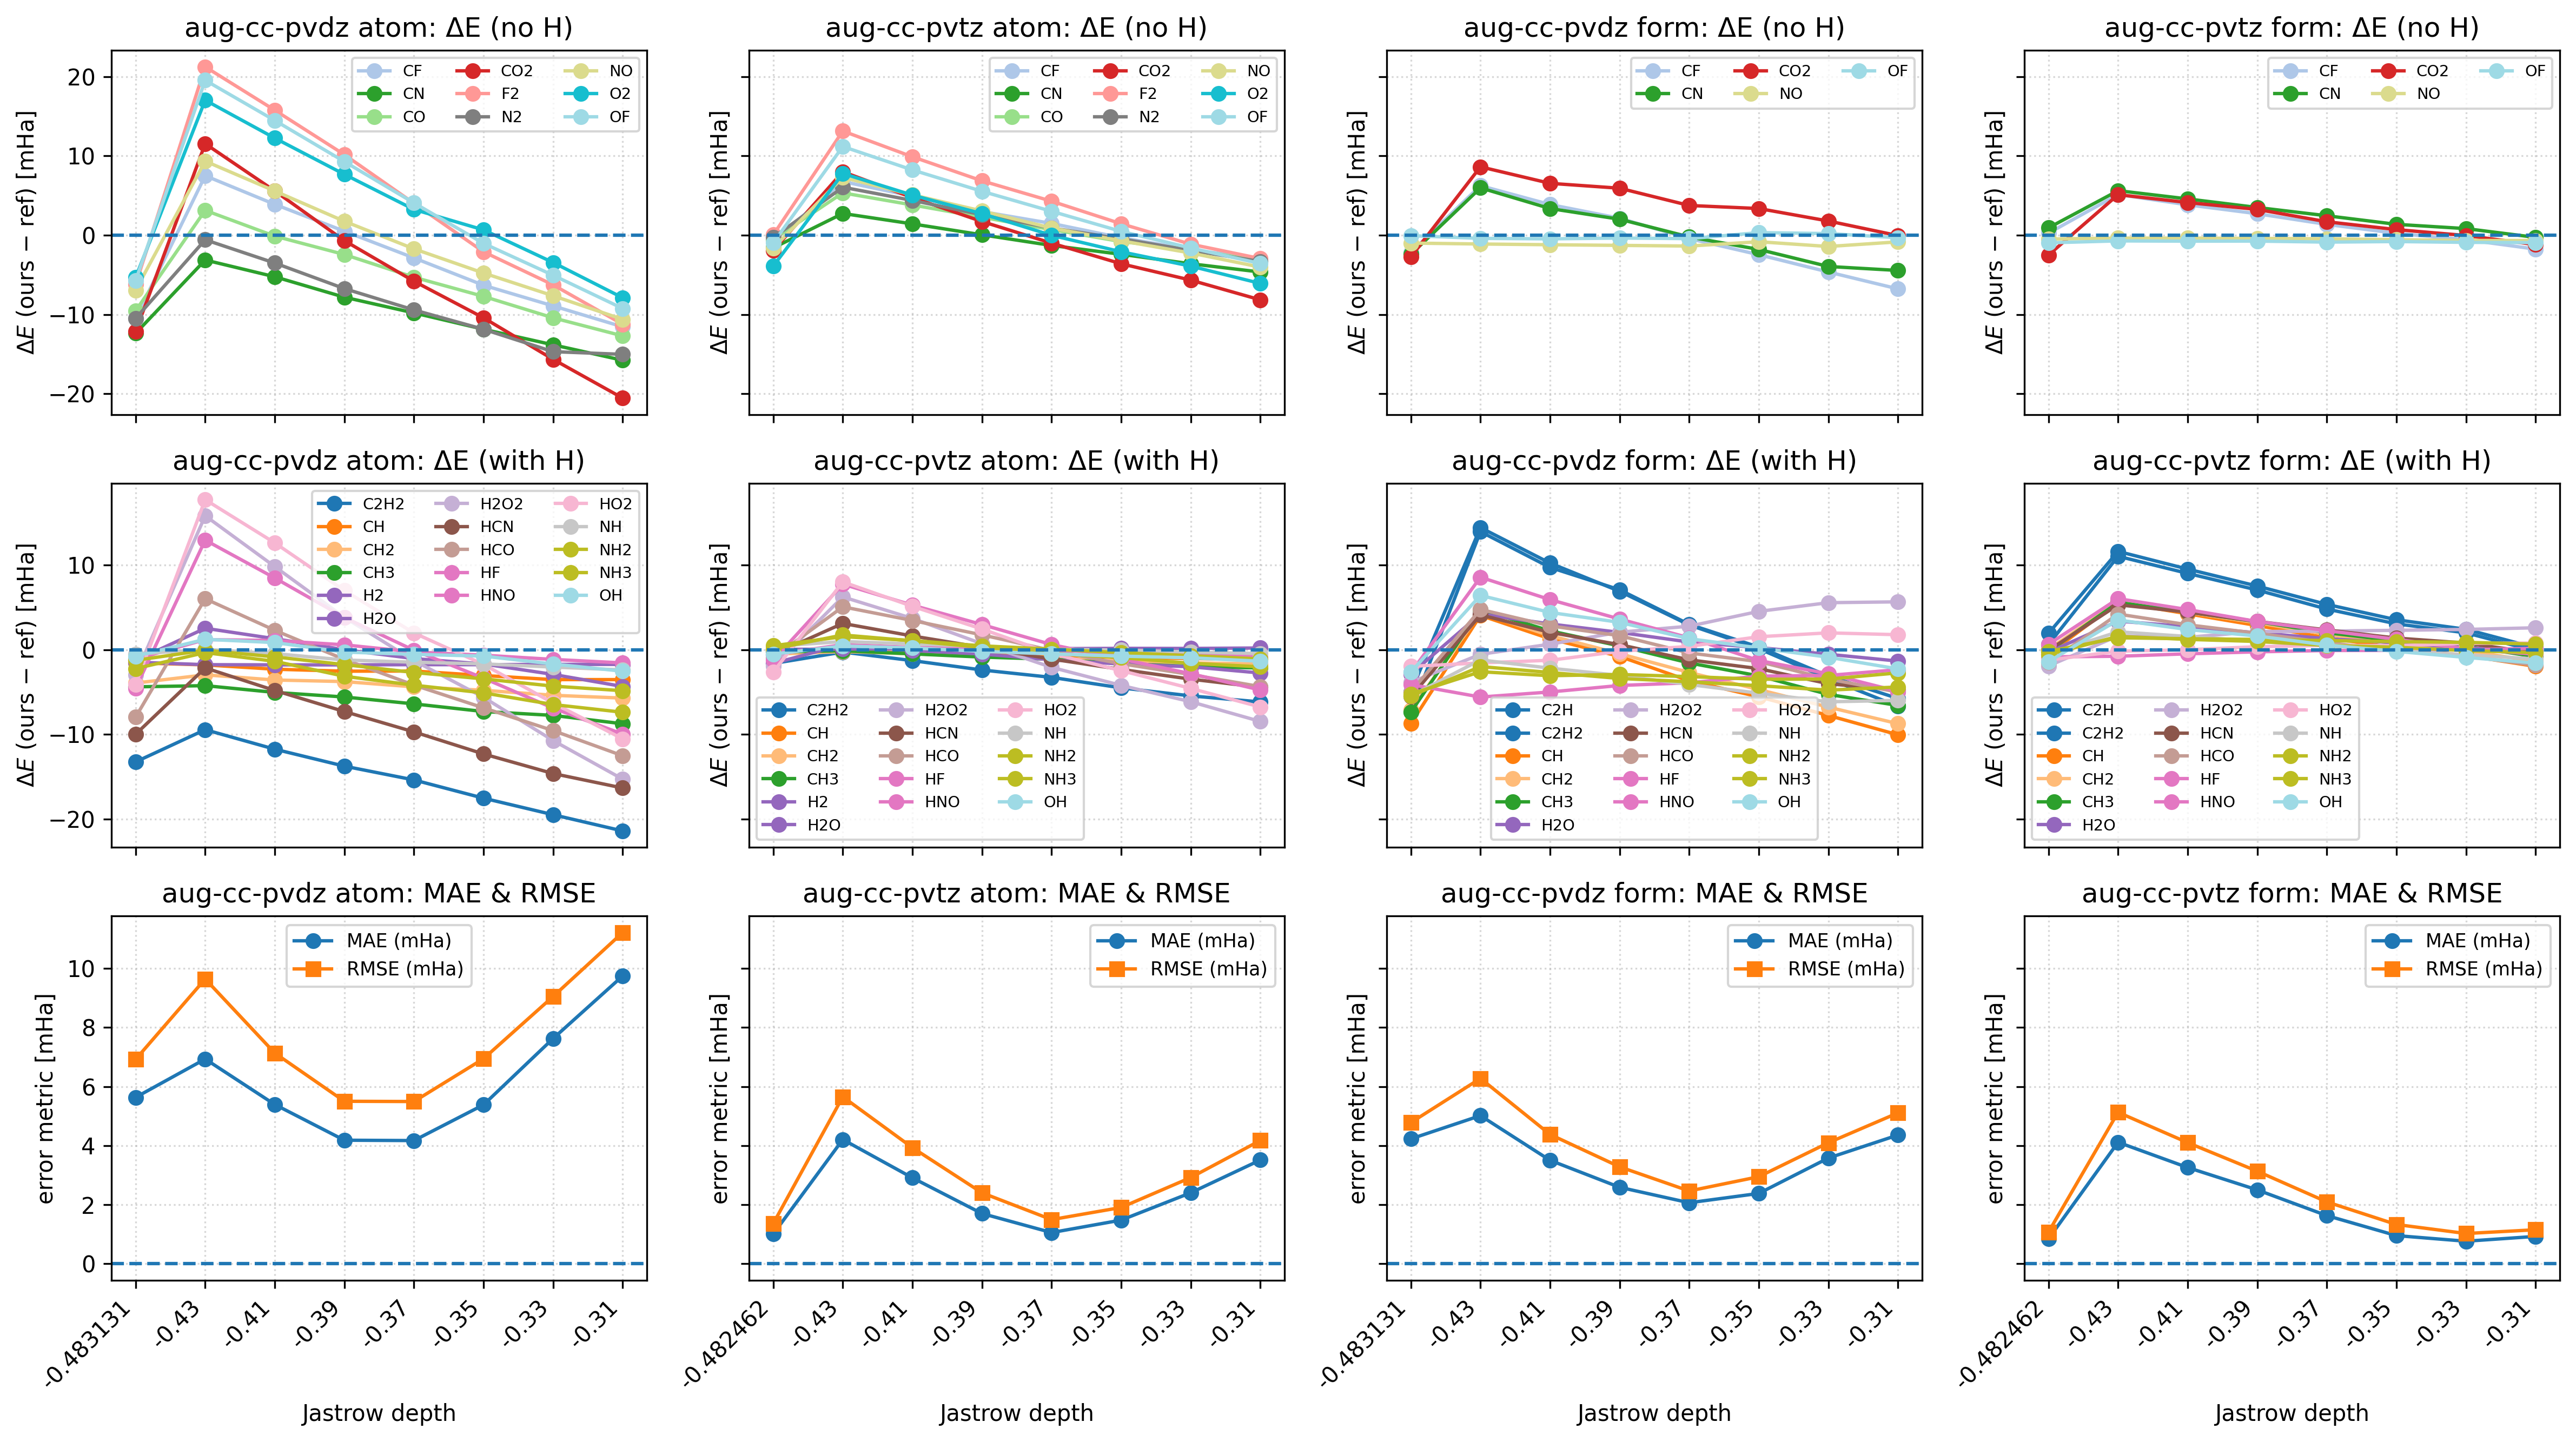
\includegraphics[width=1.1\linewidth]{figures/depth_sweep_ccECP.png}
    \caption{cECP}
    \label{fig: ccECP depth sweep}
\end{figure}
\clearpage

\subsection{Depth patterns}

\begin{figure}[htbp]
    \centering
    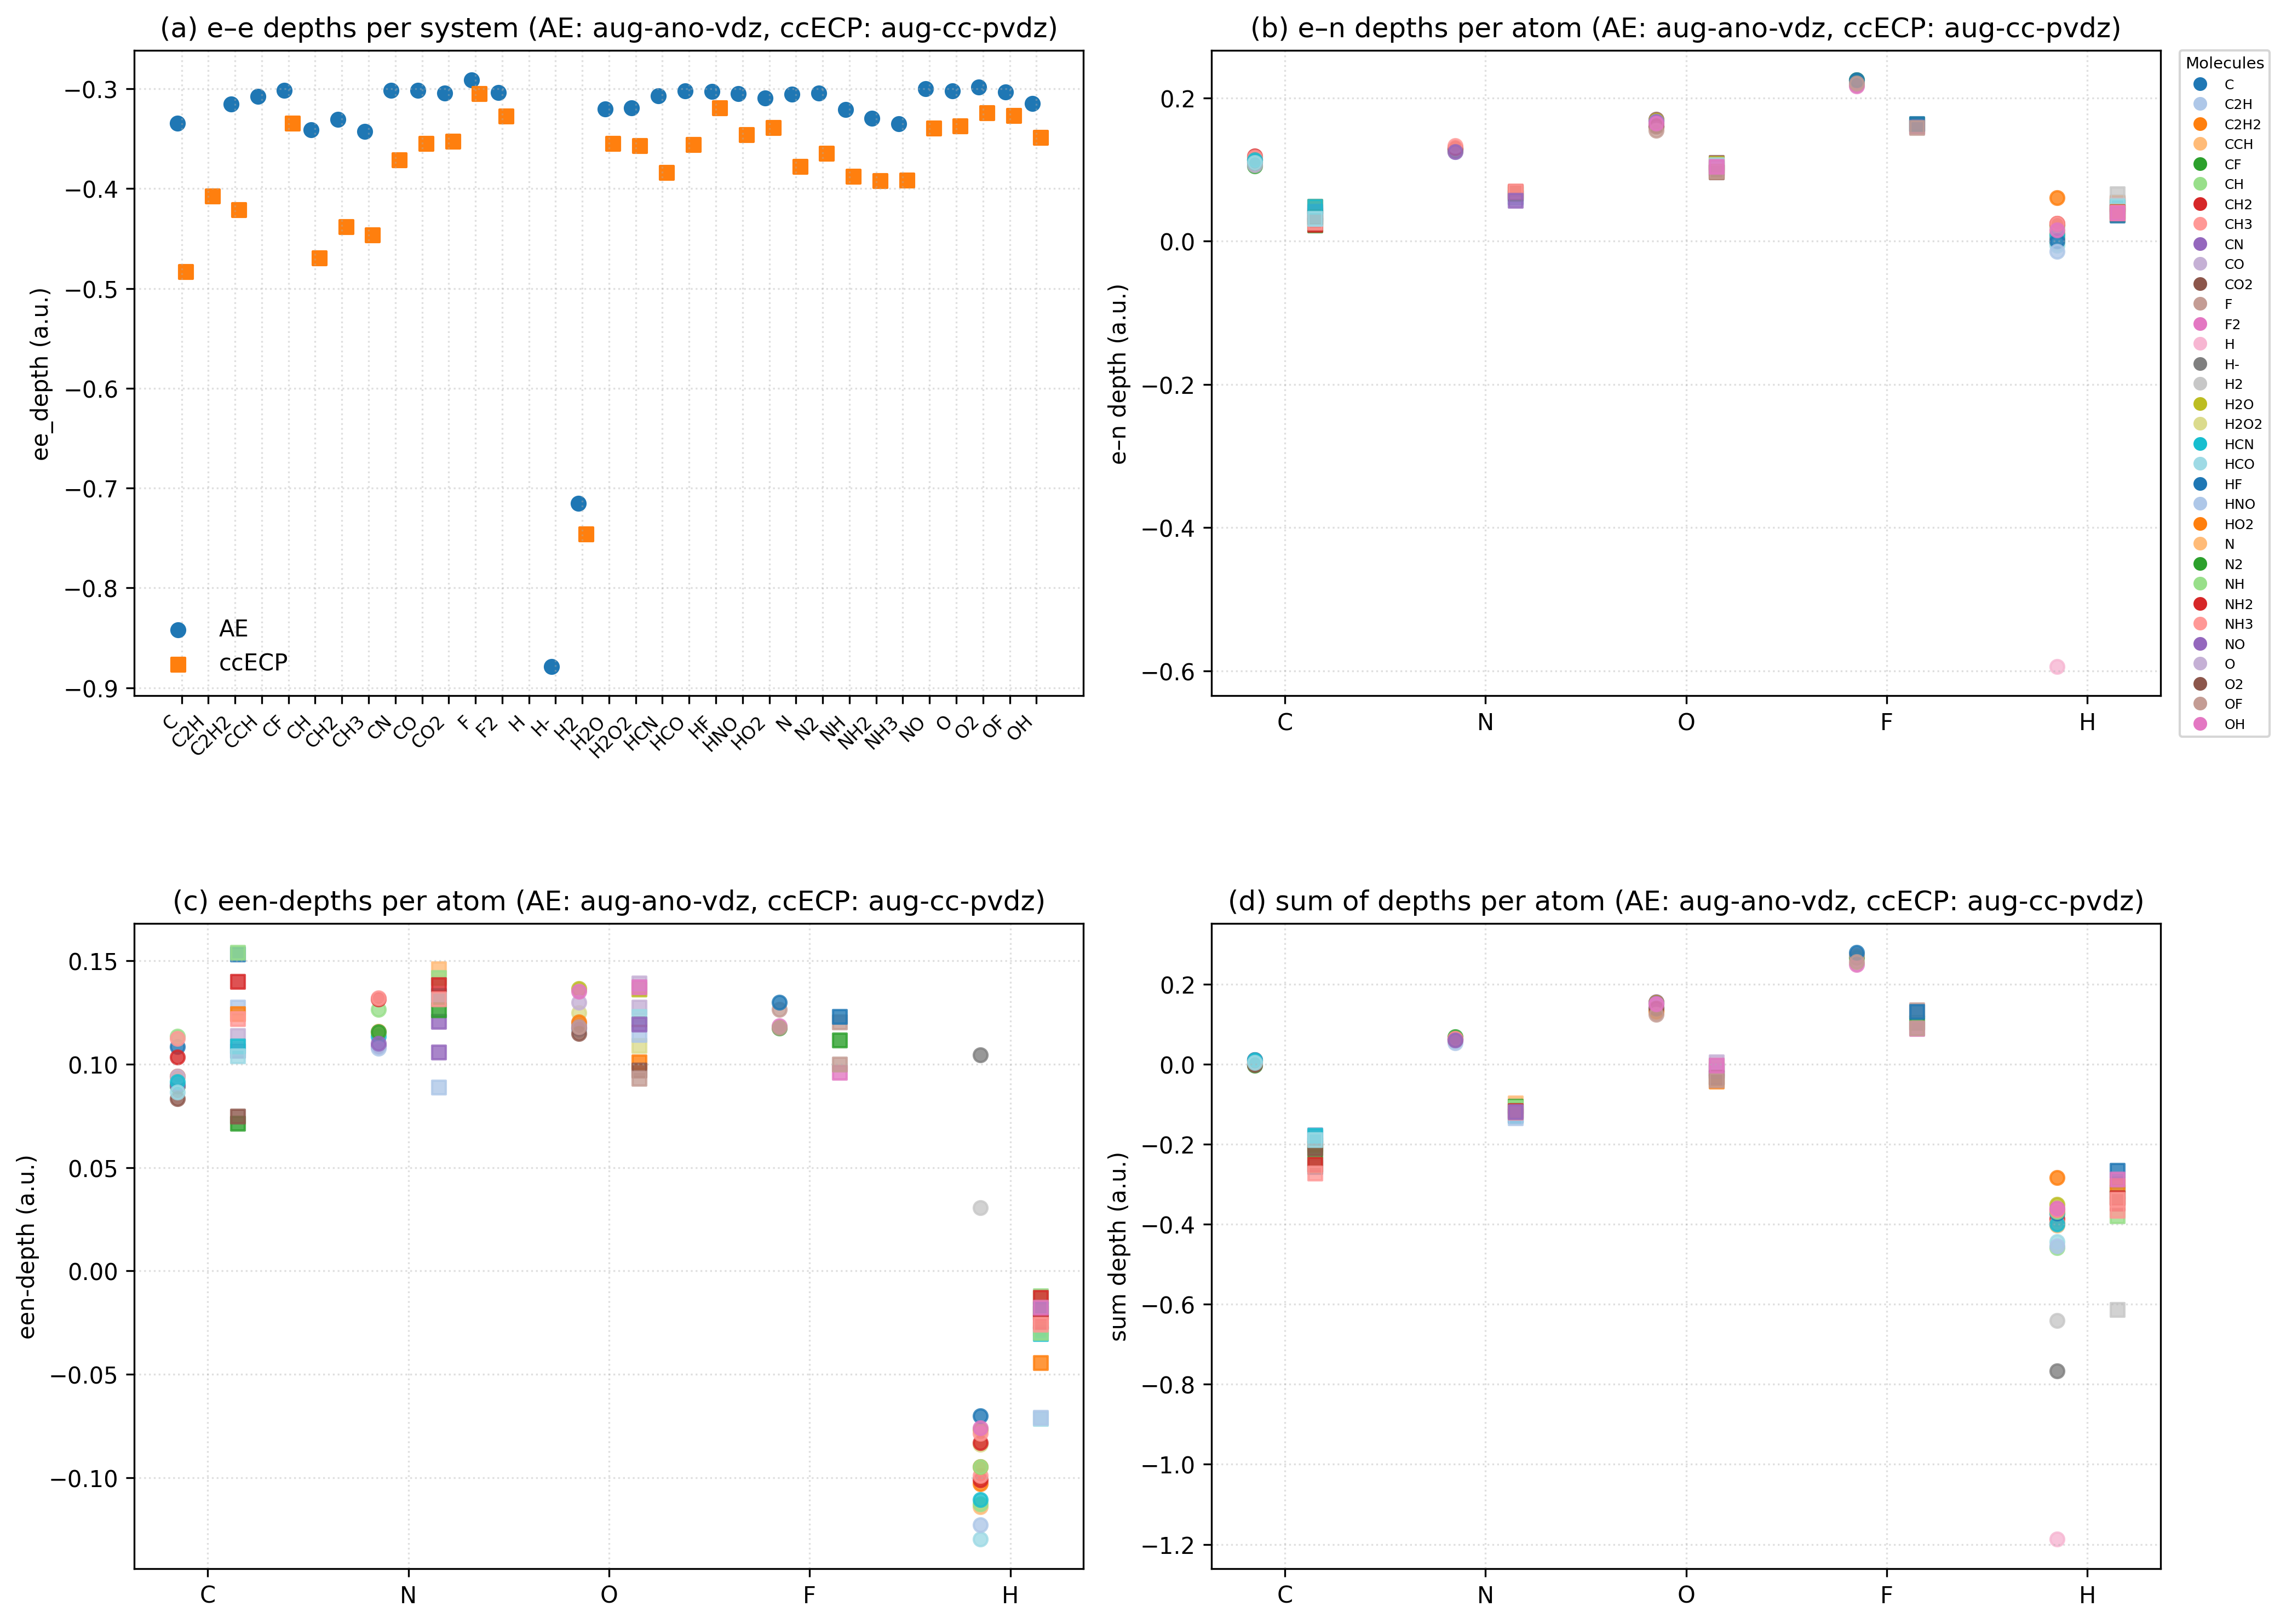
\includegraphics[width=1.2\linewidth]{figures/free_depths.png}
    \caption{Patterns of free floating depths from varmin optimizations}
    \label{fig:free depth patterns}
\end{figure}
\clearpage

\subsection{Cutoff and order sweep analysis}

We analyze the CCSD(T) versus HEAT errors (in mHa) from \texttt{data/energies\_vs\_order\_cutoff.csv}. The analyzed systems are the molecules listed in the \texttt{species} column of that file (at the moment, CH$_3$, F$_2$, HF, NH$_2$, NH$_3$). We vary the electron--nucleus and electron--electron--nucleus cutoffs ($\mathrm{en\_cutoff}$, $\mathrm{een\_cutoff}$) and the Jastrow orders ($\mathrm{ee\_order}$, $\mathrm{en\_order}$, $\mathrm{een\_order}$), and assess parameter choices by the distribution of per-system errors and by robustness across systems.

\begin{figure}[htbp]
    \centering
    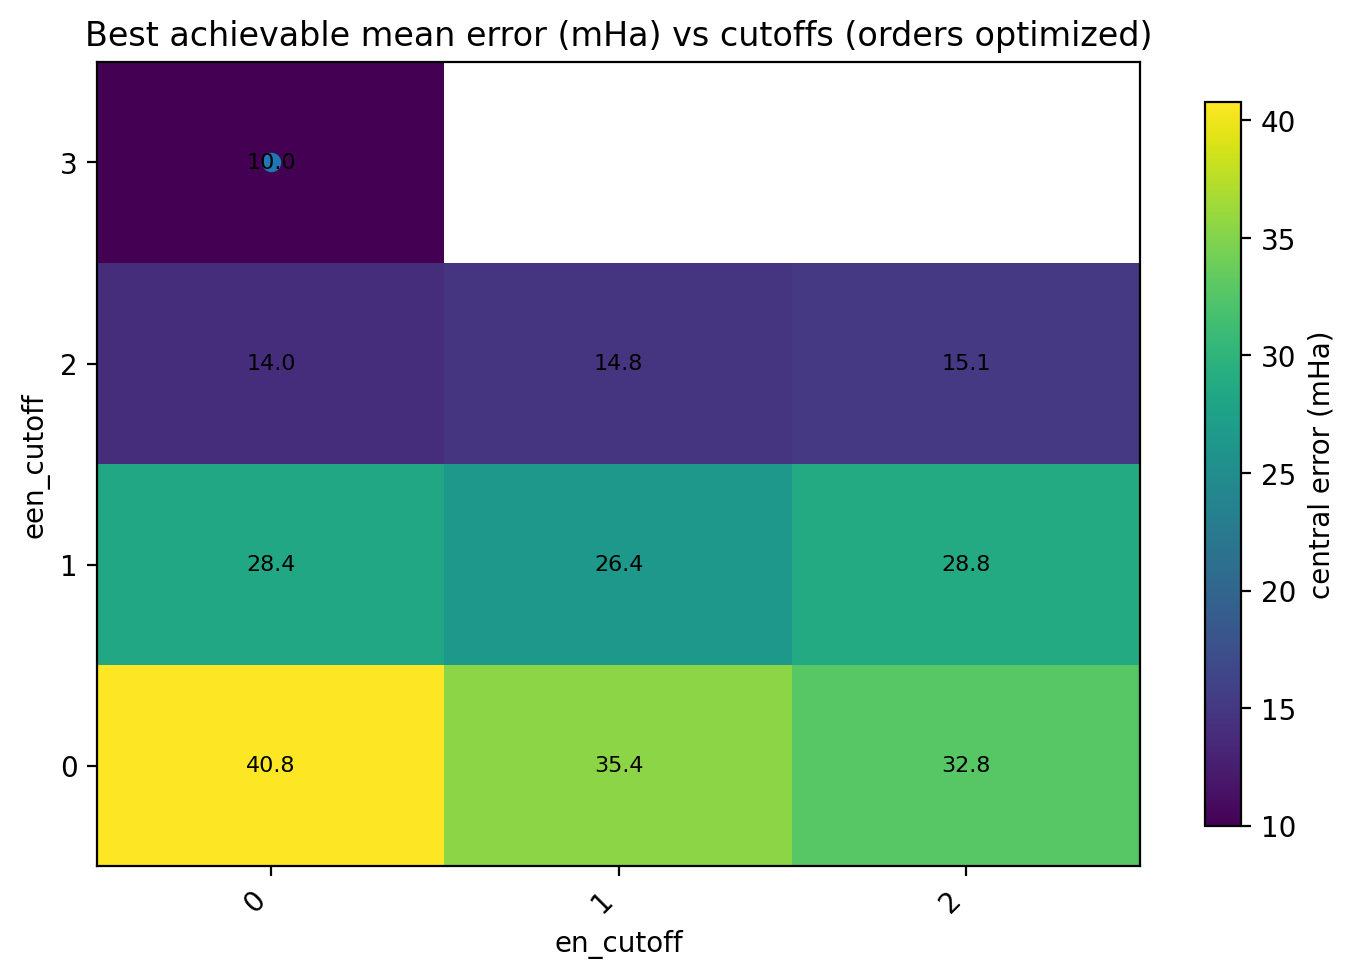
\includegraphics[width=1.05\linewidth]{figures/01_heatmap_best_vs_cutoffs.png}
    \caption{Best achievable aggregate error versus $(\mathrm{en\_cutoff}, \mathrm{een\_cutoff})$ when the Jastrow orders are varied for each cutoff pair. Cell values report the aggregate error in mHa.}
    \label{fig:cutoff_heatmap_best_vs_cutoffs}
\end{figure}

\begin{figure}[htbp]
    \centering
    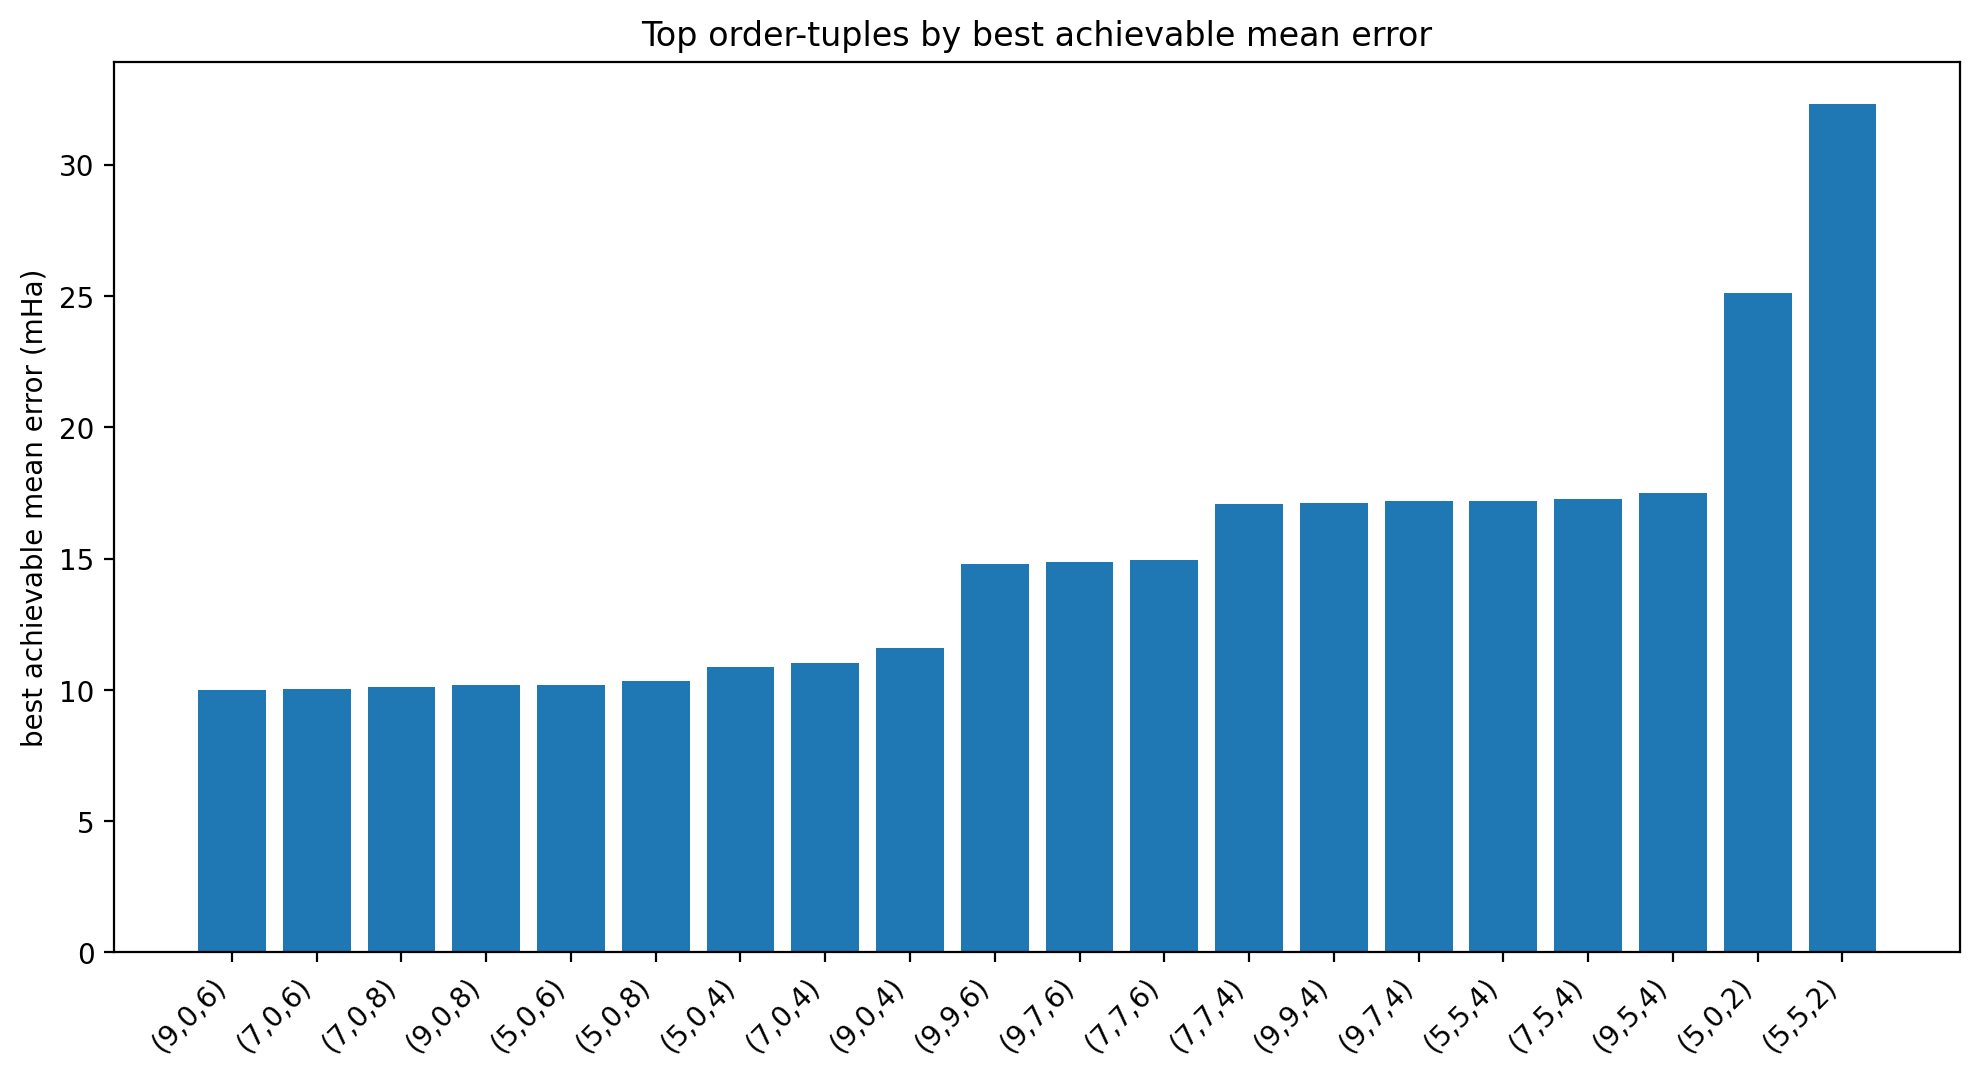
\includegraphics[width=1.05\linewidth]{figures/02_top_orders_best_possible.png}
    \caption{Best achievable aggregate error for each order triple $(\mathrm{ee\_order}, \mathrm{en\_order}, \mathrm{een\_order})$ with the tested cutoffs. Lower bars indicate better-performing order choices.}
    \label{fig:cutoff_top_orders}
\end{figure}

\begin{figure}[htbp]
    \centering
    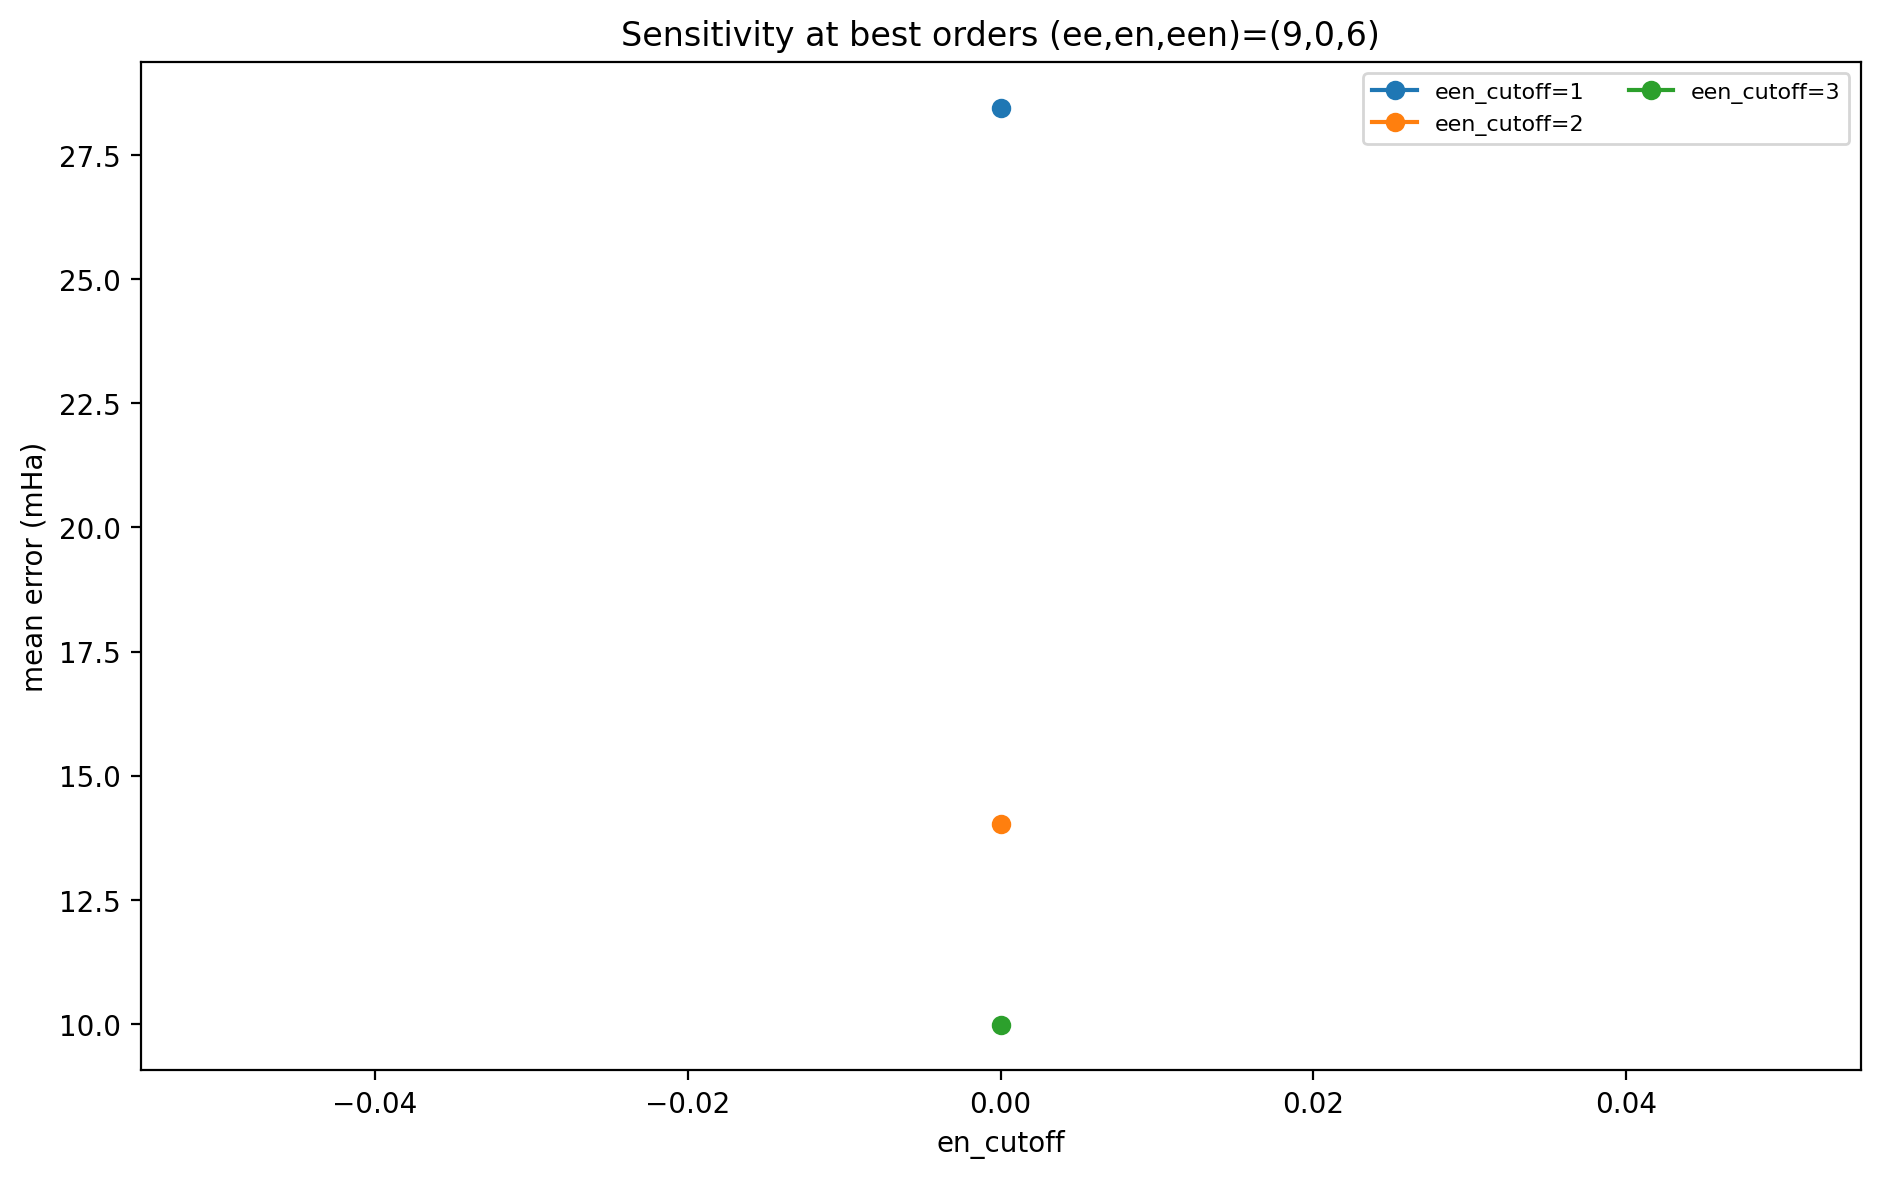
\includegraphics[width=1.05\linewidth]{figures/03_sensitivity_best_orders.png}
    \caption{Sensitivity of the aggregate error to $\mathrm{en\_cutoff}$ at the selected best order triple. Each curve corresponds to a fixed $\mathrm{een\_cutoff}$.}
    \label{fig:cutoff_sensitivity_best_orders}
\end{figure}

\begin{figure}[htbp]
    \centering
    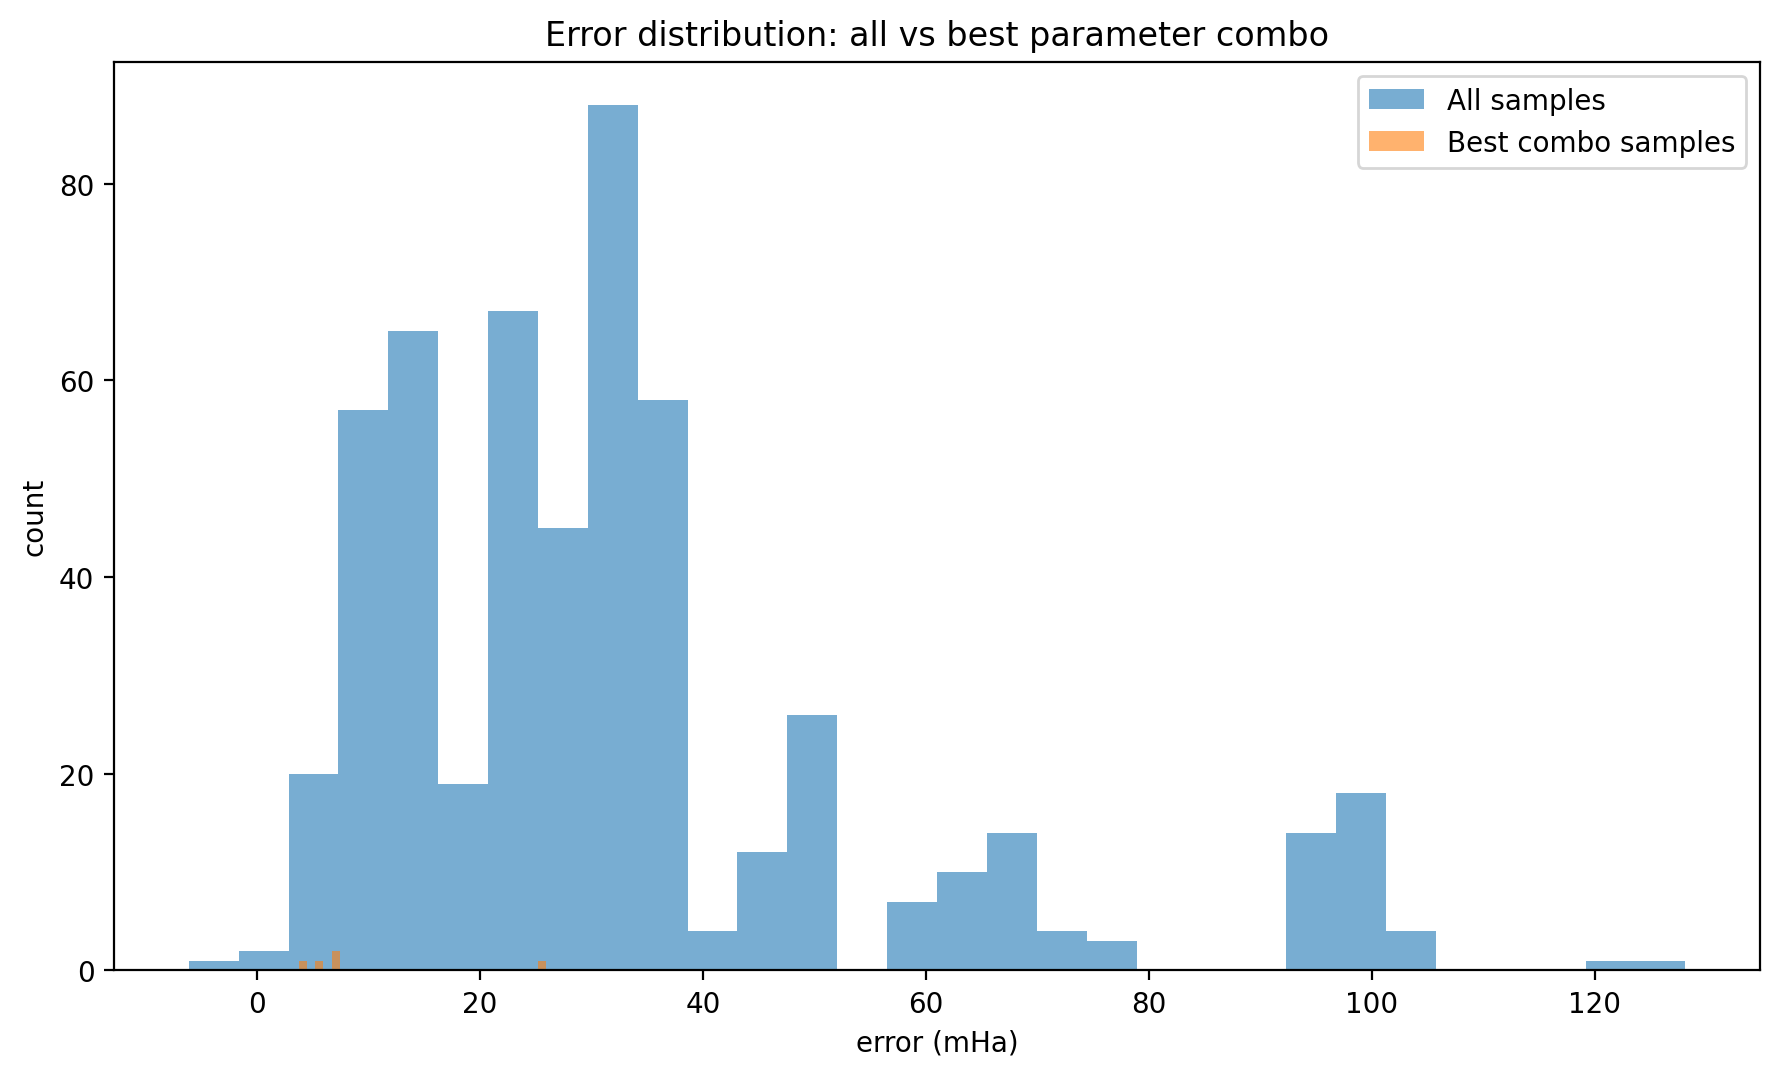
\includegraphics[width=1.05\linewidth]{figures/04_hist_all_vs_best.png}
    \caption{Distribution of individual errors (all rows in the sweep, i.e., each count denotes one molecular calculation and its error) compared to the distribution obtained at the selected best parameter combination (en cutoff=0, een-cutoff = 3, params=(9,0,6)).}
    \label{fig:cutoff_hist_all_vs_best}
\end{figure}

\begin{figure}[htbp]
    \centering
    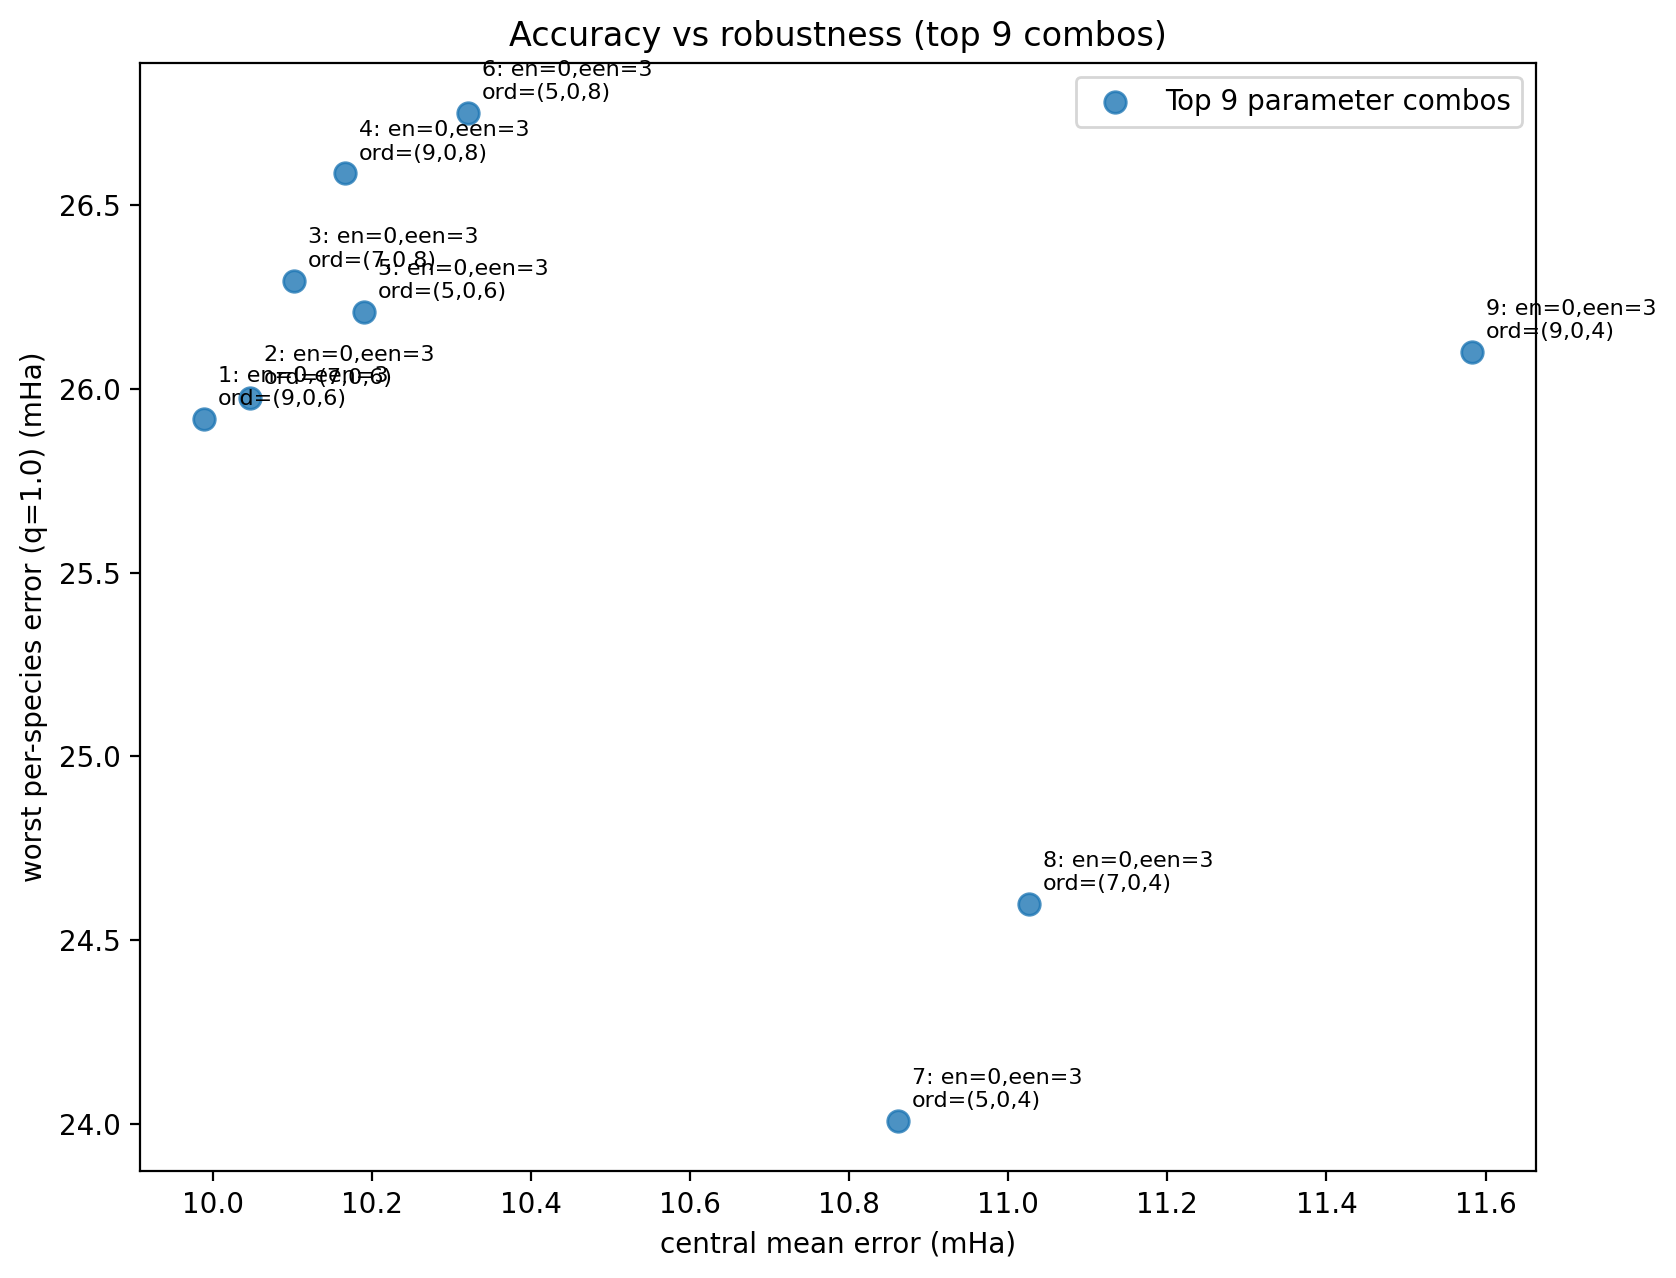
\includegraphics[width=1.05\linewidth]{figures/05_pareto_central_vs_worst.png}
    \caption{Accuracy versus robustness among the top-ranked parameter combinations. Each labeled point corresponds to one $(\mathrm{en\_cutoff}, \mathrm{een\_cutoff}, \mathrm{ee\_order}, \mathrm{en\_order}, \mathrm{een\_order})$ choice, with coordinates given by the aggregate error and the worst per-system error.}
    \label{fig:cutoff_accuracy_vs_robustness}
\end{figure}

\clearpage